\documentclass[lettersize,journal]{IEEEtran}
\usepackage{amsmath,amsfonts}
\usepackage{algorithmic}
\usepackage{algorithm}
\usepackage{array}
\usepackage[caption=false,font=normalsize,labelfont=sf,textfont=sf]{subfig}
\usepackage{textcomp}
\usepackage{stfloats}
\usepackage{url}
\usepackage{verbatim}
\usepackage{graphicx}
\usepackage{cite}
\usepackage{tabularx}
\usepackage{boldline}
%\usepackage[justification=centering]{caption}
%\usepackage{hyperref}
\hyphenation{op-tical net-works semi-conduc-tor IEEE-Xplore}
% updated with editorial comments 8/9/2021

\begin{document}

\title{Power System Transient Stability Simulation Results Compression Method}

\author {Eugene Mashalov, Joint Stock Company "Scientific and Technical Center of Unified Power System", Ekaterinburg, Russia}


%\markboth{Journal of \LaTeX\ Class Files,~Vol.~14, No.~8, August~2021}%
%${Shell \MakeLowercase{\textit{et al.}}: A Sample Article Using IEEEtran.cls for IEEE Journals}

%\IEEEpubid{0000--0000/00\$00.00~\copyright~2021 IEEE}
% Remember, if you use this you must call \IEEEpubidadjcol in the second
% column for its text to clear the IEEEpubid mark.

\maketitle

\begin{abstract}
Transient stability analysis simulation software can produce large amount of
the resulting data, representing the time series of parameters. Modern power system models
are highly detailed, and the duration of simulation is usually tens of minutes. 
In addition, power system simulations is generally performed on multiple variants with
varying model parameters. The resulting time series for tens of thousands of variables
may require significant storage and its cost may be tangible even for modern computer systems.
This article discusses the compression algorithm and its implementation, which can 
losslessly reduce the amount of time series data by about 40\% with small computational overhead.
\end{abstract}

\begin{IEEEkeywords}
Power System Transient Stability Simulation, Time Series Lossless Compression.
\end{IEEEkeywords}

\section{Introduction}
\IEEEPARstart{M}{odern} power system transient stability analysis practice is mainly involved
into development of new facilities and also plays a significant role in post-contingency
control. The last task requires just single answer to the question "will this contingency be stable or not ?"
Simple criteria, such as angle or energy based can be used to evaluate transient stability, and in 
most cases they do not require time series analysis. But for system setup, tuning and incident inquiries
detailed time series are still required. With regard to development tasks, time series are most important
supplement material for design documentation and their study requires at least all machine angles, 
voltage magnitudes and angles of buses, some control signals. In most cases much more data should be presented. 
Thus, the ability to store large amount of transient stability time series should be provided, at least optionally.

The resulting time series are snapshots of model state variables at arbitrary moments of transient.
The sampling rate of snapshots is uneven and conditioned by integration step. Dense output is not used often, as it 
produces excess data for long-term transients decay phases. Some model variables have discrete nature, such
as breaker positions and network parameters changes. Their dense representation also inefficient.

\begin{table}[!h]
	\caption{State variable count for basic transient stability equipment models\label{tab:statvarscount}}
	\centering
	\begin{tabularx}{\columnwidth}{l|X|r}
		\hline
		Model & Description & Count\\
		\hlineB{3}	
		Bus & Voltage angle and magnitude, filtered voltage slip & 4\\
		\hline
		Load & Active and reactive power & 2\\
		\hline
		Generator & Simplified generator model with active and reactive power, voltage and current on dq-axes, 
		angle, slip, transient and excitation EMFs & 10\\
		\hline
		Exciter & Voltage at bus, output & 3\\
		\hline
		AVR & Excitation EMF, voltage, slip and excitation current filtered derivatives, output, filtered slip & 12\\
		\hline
		DEC & Discrete excitation control: 2 relays, 2 triggers, voltage magnitude & 7\\
		\hline
	\end{tabularx}
\end{table}

To get an idea of the amount of data to be stored consider the number of state variable for basic transient 
stability equipment models in the table \ref{tab:statvarscount}. The equipment models used are not 
highly detailed, but overall practical model dimension gives 6624 state variables. For 60s simulation with
output step \(10^{-2}\)s and double precision representation of results the required amount of memory will be 303.2MB.
Of course output can be limited to a selected set of state variables to reduce storage requirements,
but this selection require extra care for various cases of contingencies.

The storage required for resulting time series depends on model dimension, simulation duration
and accuracy, as well as transient response features. State variables values are computed on each DAE integration
step \(h\), but the results go to output with much slower rate than integration step \(H_p>>h\). 
When integration uses \(h<H_p\), intermediate instants in \([t;t+H_p]\) are not stored, except
instants with discrete events, such as switching, limiting and contingencies. At discrete instants
results are stored before the event in \(t_d^-\) and after the event in \(t_d^+\), \(0<t_d^+-t_d^-<h_{min}\).
Such a representation is much more convenient for the analysis of discrete events, since it preserves
discontinuity, but it also increases the amount of data stored, and it grows in proportion to the 
frequency of discrete events.

When transient decays, state variables amplitude oscillations become smaller, which increases
integration method extrapolation accuracy and allows to increase \(h\) appropriately.
When \(h>H_p\) result output will use \(h\) instead of \(H_p\). If transient decay is slow or
transient is unstable its simulation results will require much more storage, as integration
step is unlikely to reach \(H_p\). 

Low-precision transient simulation with limited error tolerances requires less memory since \(h\) can usually be
greater than \(H_p\), but the quality of the simulation cannot be considered as a storage reduction factor.

\section{Transient stability results features and general purpose compression algorithms}
Consider the simulation results time series as subject to data compression:

\begin{enumerate}
	\item{Simulation results are sequential time series. In most cases they are approximations
	to piecewise smooth functions, which are DAE solutions. The difference of two successive
	values are small, suggesting high data redundancy.}
	\item{All time series values are associated with common time values. It can be used to store the only time data for all series.}
	\item{Some state variables are discrete or change infrequently. This is also true for state variables that have reached their limits. The values of these state variables remain fixed for a relatively long period of simulation time or vary within a small range of integration accuracy.}
	\item{When the transient decays, most state variables tend to steady state with negligible oscillations.}
	\item{Any state variable can be subject to discontinuity due to discrete event. It is assumed that discrete events frequency is limited in most cases. }
\end{enumerate}

When data compression is needed one of many available commercial or free software libraries can be used.
Most of data compression algorithms are general purpose, and do not consider data features.
Data compression is based on redundancy detection and removal \cite{lzw77,welch84}. 
Some methods use preconditioning to improve further compression ratios \cite{bwt94} or dictionaries 
with most frequently occurring data sequences.  All of these algorithms assume that the data to be compressed is
fully available or available by relatively large successive blocks. Decompression assumes 
lossless restoration of the original data from the compressed and also operates on full data set. 
This leads to memory requirements to fit data to be processed.

Transient stability simulation results may contain data for tens of thousands of state variables.
Depending on the engineering problem, a large subset of them may need to be worked on, but it is unlikely that a complete set of data will be required.
Thus, it is desirable to be able to decompress only a subset of the results for selected state variables. 
In order to achieve this capability from the general purpose algorithms, it is necessary to compress the data for each 
state variable separately, which will lead to an increased CPU, memory and storage overhead.

The above peculiarities of general purpose algorithms make them less efficient for simulation 
results compression. General purpose algorithms should be adapted to work on time series. 
The table \ref{tab:gpcompr} shows relationships between simulation results features, general purpose
compression algorithms peculiarities and possible workarounds to use algorithms to work with
results.

\begin{table}[!h]
	\caption{General purpose compression for simulation results\label{tab:gpcompr}}
	\centering
	\begin{tabularx}{\columnwidth}{ 
			  >{\raggedright\arraybackslash}X 
			| >{\raggedright\arraybackslash}X 
			| >{\raggedright\arraybackslash}X }
		\hline
		Results feature & General Purpose compression peculiarity & Workaround\\
		\hlineB{3}	
		Available sequentially as integration progresses & 
		Requires access to full data set or it's large parts  &
		Intermediate buffer to accumulate results to be compressed\\
		\hline
		Access to selected results & 
		Restores full compressed dataset & 
		Much more data should be decomressed than needed\\
		\hline
	\end{tabularx}
\end{table}

One can consider separate compression of each time series or their groups by
general purpose algorithms. This approach will require separate instances
of the algorithm as well as increase amount of memory required. For time series
consisting of thousands of separate channels memory amount may be inappropriate.

There are compression algorithms designed for specific data. Lossless audio compression
algorithms, for example, work actually on time series \cite{lch03}. But those 
algorithms are designed for fixed sample rates and integer sample values, 
which is not the case for simulation results. Audio compression works well
with multiple channels, but not with thousands of simultaneous separate channels,
due to performance penalties. A high compression ratios achieved by trying
several compression methods and further best ratio selection. This also may
lead to performance drop.

Data compression performance is one of most important features to be considered.
When data compression is used for transient stability simulation results it
is auxiliary function, as system resources must be used for computation. 
A reasonable approach is to run result compression in separate process/thread and 
give it enough CPU time to process the computed results while computing the next results.
Thus system resources will be optimally distributed and synchronization bottlenecks will be avoided.

\section{Transient stability simulation results compression algorithm}
Besides algorithms reviewed above which are suitable for compressing general or media data,
there are algorithms designed for scientific data exchange. The are widely used for MPI systems \cite{camata10}. 
When the bandwidth is limited data compression can improve performance even at additional
cost on processing.
These algorithms are designed for 32- or 64-bits floating point values and exploit encoding
scheme for IEEE-754 numbers. Consider 64-bit value pattern:

\begin{table}[!h]
%	\caption{IEEE-754 64 bit floating point number format\label{tab:gpcompr}}
	\centering
	\begin{tabularx}{\columnwidth}{ 
		 	| >{\raggedright\arraybackslash}X 
			| >{\raggedright\arraybackslash}X 
			| >{\raggedright\arraybackslash}X 
			| >{\raggedright\arraybackslash}X |}
		\hline
		Bits & 63 & 62-52 & 51-0\\
		\hline
   	    Purpose & Sign & Exponent & Mantissa\\
		\hline
	\end{tabularx}
\end{table}

Let \(a\) and \(b\) be floating point numbers, and \(a\approx b\). This means most exponent and most of mantissa 
bits will match between \(a\) and \(b\). If we compute exclusive or \(c=a \oplus b\) the high bits of \(c\) will
be zero. Higher non-zero bits count in \(c\) will decrease as \(a\) approaches to \(b\). If one can count
higher non zero bits, \(c\) can be represented with the following encoding scheme:

\begin{table}[!h]
%\caption{Floating point number encoding by exclusive or}
	\centering
	\begin{tabularx}{0.2\columnwidth}{ 
			| >{\centering\arraybackslash}X 
			| >{\centering\arraybackslash}X |}
		\hline
		\(Z_B\) & \(C_B\)\\
		\hline
	\end{tabularx}
\end{table}

\noindent where \(Z_B\) it the number of zero bits divided by 4, \(C_B\) is non-zero bits sequence.
To store \(Z_B\) 4 bits are needed. To store \(C_B\) --- \(64 - 4*Z_B\) bits. 
Since \(\oplus\) reversible, the original \(a\) can be restored by \(a = c \oplus b\) with \(c\)
and \(b\) casted to the IEEE-754 bit pattern. It can be seen that encoding and decoding are lossless.

Consider the example of encoding \(a \approx \pi\) up to 16 decimal digits. Let \(b\approx \pi\) 
up to 10 decimal digits. The IEEE-754 representation of \(a\) and \(b\) is as follows:

\begin{table}[!h]
%	\caption{Floating point number encoding by exclusive or}
	\centering
	\fontsize{5.5}{1.2} {
	\begin{tabularx}{\columnwidth}{ 
			| >{\raggedleft\arraybackslash}l 
			| >{\raggedright\arraybackslash}X |}
		\hline
		 \(a\) & \texttt{0100000000001001001000011111101101010100010001000010110100011000} \\
		\hline
		\(b\) & \texttt{0100000000001001001000011111101101010100010000010001011101000100} \\
		\hline
	\end{tabularx}
}
\end{table}

The resulting \(c=a \oplus b\) is:

\begin{table}[!h]
	%	\caption{Floating point number encoding by exclusive or}
	\centering
	\fontsize{5.5}{1.2} {
		\begin{tabularx}{\columnwidth}{ 
				| >{\raggedleft\arraybackslash}l 
				| >{\raggedright\arraybackslash}l 
 			    | >{\raggedright\arraybackslash}X |}
			\hline
			\(c\) & \texttt{00000000000000000000000000000000000000000000} & \texttt{01010011101001011100} \\
			\hline
		    & \multicolumn{1}{c|} {\(Z_B * 4\)} & \multicolumn{1}{c|} {\(C_B\)} \\ 
			\hline
		\end{tabularx}
	}
\end{table}

Since \(c\) has 45 higher zero bits, \(Z_B\)=11. The encoded form of \(c\) would then be:

\begin{table}[!h]
	%	\caption{Floating point number encoding by exclusive or}
	\centering
	\fontsize{5.5}{1.2} {
		\begin{tabularx}{0.4\columnwidth}{ 
				| >{\raggedright\arraybackslash}l 
				| >{\raggedright\arraybackslash}X |}
			\hline
			\multicolumn{1}{|c|} {\(Z_B\)} & \multicolumn{1}{c|} {\(C_B\)} \\ 
			\hline
			\texttt{1011} & \texttt{01010011101001011100} \\
			\hline
		\end{tabularx}
	}
\end{table}

To store \(a\) 24 bits required instead of 64. The compression ratio \(K_c=24/64=0.375\). 
Decoding of \(a\) can be done in reverse order.

An encoding scheme can be applied to floating point numbers sequence \(a_i\), if one can generate sequence \(b_i\)
with values close enough to \(a_i\) values. Assume function \(f(i)\), whose values sufficiently close to \(a_i\).
In \cite{ratana06} this function is called predictor and it is based on DFCM algorithm, used for prediction of cache operations for microprocessors. The function algorithm successively builds a hash table of previous sequence values differences. 
With a sufficient hash table size algorithm can predict repeating patterns in the data sequence. Compression
algorithm with predictor is shown in Fig \ref{fig_compr}.

\begin{figure}[h]
	\centering
	
\includegraphics[width=0.8\columnwidth]{fig1.eps}
	\caption{Compression algorithm.}
	\label{fig_compr}
\end{figure}

To compress \(a_i\) in the sequence of \(a_i=a(t_i)\) the predictor generates \(b_i\) to compute 
\(c=a \oplus b \). 
Then \(Z_{bi}\) is determined by counting higher zero bits of \(c_i\) and encoded pair \(Z_{bi}\), \(C_{bi}\) then ready to store.
Predictor is updated with \(a_i\).

\begin{figure}[h]
	\centering
	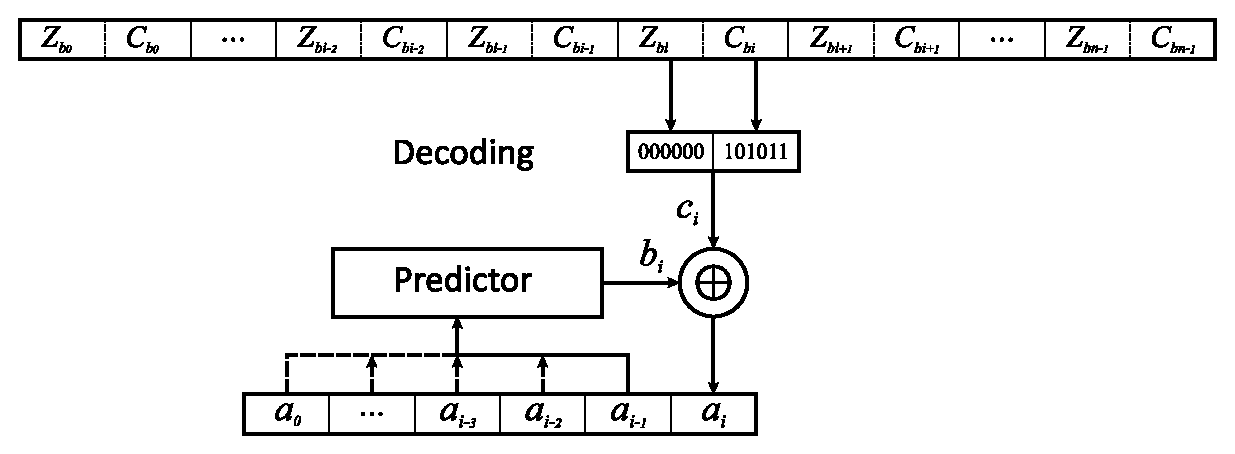
\includegraphics[width=0.8\columnwidth]{fig2.eps}
	\caption{Decompression algorithm.}
	\label{fig_decompr}
\end{figure}

To decompress \(a_i\) from the stored sequence \(c_i\), the encoded pair \(Z_{bi}\), \(C_{bi}\) 
is mapped to IEEE-754 bit pattern. Predictor generates \(b_i\) and \(a\) restores by XOR operation.
Predictor is updated with \(a_i\). The \(b_i\) sequences generated by the predictor for encoding and decoding are the same, as they use the same \(a_i\).

The closer \(b_i\) given by the predictor function, to the original values of \(a_i\), the better compression ratio can be obtained. 
Therefore, the predictor function should consider the most of the features of the data being processed. 
A hash table-based predictor suits for general floating point periodic data. It automatically adjusts to the processed sequence and, if a period can be distinguished in the data, it provides high accuracy of the forecast. 
However, the use of a hash table comes with a major disadvantage of such a predictor, since 
its storage requires memory (about 16MB for optimal prediction quality at transient simulation duration over 60s). 
In the considered problem of compression of the results of transients simulation, an individual hash table must be created for each state variable.

It was noted above that simulation results  in most cases are approximations to piecewise smooth functions.
This property gives option to use Lagrange polynomial extrapolation for prediction:

\begin{equation}
	\label{eqn_lagrb}
	b_i=b_i(t_i)=\sum_{m=1}^{np+1} a(t_{i-m})l_m(t_i),
\end{equation}
\noindent with basis polynomials:
\begin{equation}
	\label{eqn_lagrbasic}
	l_m(t_i)=\prod_{k=1, k \neq m}^{np+1} \frac{t_i-t_{i-k}}{t_{i-m}-t_{i-k}}
\end{equation}

\noindent where \(np\) is the order of the polynomial, which also the order of predictor. 
The Lagrange polynomial does not require \(t_i\) to be equally spaced. This property allows to output
the results from integration method directly without dense output processing.

The prediction method used for encoding is similar to the prediction method for DAE integration. 
For such a predictor to work, it is sufficient to have a vector of previous values with a depth equal to the order of the predictor. 
The order can be changed, if necessary, at virtually no additional cost. 
Increasing the order of the predictor improves the quality of prediction for high-order components of transient. 
Considering also that all values of the results are related to common time values, the basis polynomials \ref{eqn_lagrbasic} can be calculated once 
for all state variables that going to output at the current step \(t_i\). Thus, for the results, it is optimal 
to choose a predictor with Lagrange extrapolation, which requires a negligible amount of memory and makes it possible to eliminate redundant computations.

The order of the predictor polynomial can vary from zero to some \(n_{Pmax}\). For the first step of transient stability simulation, the value of the DAE
initial conditions is used as the predictor value. The next step gives a linear extrapolation, and so on. 
It has been found empirically that the best compression ratio gives the value \(n_{Pmax}=4\). A the order increases prediction worsens. Presumably, the reason for this is the Runge phenomenon, since most of the results are stored with a step \(h_P\), with slight deviations.

As noted above, for discrete changes, the time instants \(t_d^-\) and \(t_d^+\) are preserved. 
Since \(t_d^- \neq t_d^+\), the proposed compression method  remains operational, but at the instants of 
discrete changes it can degrade the compression ratio, as the function undergoes a discontinuity 
and polynomial extrapolation cannot give a qualitative prediction. In the instants of discrete changes, 
the integration stops and new initial conditions are calculated for \(t_d^+\), 
after which the integration resumes. The order of the predictor after calculating the new initial conditions is reset to zero and increases 
to \(n_{Pmax}\) as new integration results are accumulated. This approach to processing discrete changes allows to maintain an acceptable compression ratio, since it takes into account the discontinuity of the function of the simulation result.
 
With an exact match between the predicted and stored value of the simulation result, the encoding scheme allows to reduce the
representation to 1 byte - F0 (in hexadecimal), while \(K_c=0.125\). Such prediction accuracy is unlikely for time-varying parameters, 
but for piecewise constant parameters such as outputs of discrete elements, or parameters that are at the limits, this is easily achievable. 
Taking into account the fact that the time intervals during which the values of such parameters do not change can be long, 
it is possible to further improve the compression ratio by using Run Length Encoding (RLE). 
Before saving, the results compressed by the proposed method are accumulated in a fixed size buffer with a repetition counter. 
If the buffer is not empty and the value of the current calculation result is the same as the previous one, the current value 
is not written to the buffer, but instead the repeat counter is incremented. Thus, a series of repeating consecutive values is 
encoded by the given value and the number of its repetitions.
If the repeat counter has a non-zero value, but the previous and current values of the calculation result do not match, 
the contents of the buffer are stored, after which the buffer size and the repeat counter are reset to zero values.

The simulation results when using additional run-length encoding are stored in the form of blocks. 
The block is marked with a repeat counter. If the repetition counter is zero, then the block contains non-repeating 
data compressed by the proposed method. Otherwise, the block contains a series of equal values that can be recovered 
by decoding the single value and copying it in sequence. The buffer size within 50-100 samples does not lead to a significant memory consumption, but allows I/O operations to process more data, which increases write speed when saving results to file
and the speed of access when reading and restoring results for viewing and analysis. 
File I/O operations, both read and write, are sequential.

The proposed compression method provides exact data recovery, that is, it is a lossless compression method. 
This property of the algorithm is valuable, but it is redundant for storing the results of 
transient stability simulation, as it is carried out with the finite accuracy of the integration method. 
The local error is controlled by predictor-corrector integration scheme:
\begin{equation}
	\label{eqn_interror}
	d_i=C\frac{e_i}{|y_i|Rtol+Atol} \leq 1
\end{equation}

\noindent where
\begin{description}
	\item  \(e_i\) is the corrector equation error with respect to the 
	state variable \(y_i\);
	\item  \(C\) is a constant of the integration method;
	\item  \(Rtol\) is the relative error tolerance;
	\item  \(Atol\) is the absolute error tolerance.
\end{description}

Obviously, limiting the accuracy while storing the simulation results 
to the value of \(Atol\) will not lead to a deterioration in the quality of the transient stability analysis. 
Therefore, a preliminary filter can be applied, which rounds values to \(Atol\). 
Filtering by itself does not provide compression, but allows to get the result in the form of a piecewise
constant function and use run-length encoding for intervals in which the change in the result value does not exceed \(Atol\), as shown on Fig. \ref{fig_rle}. 
Filtering does not introduce an additional error into the simulation 
result and does not affect the quality of the analysis of the simulation result, but improves compression ratio.

\begin{figure}[h]
	\centering
	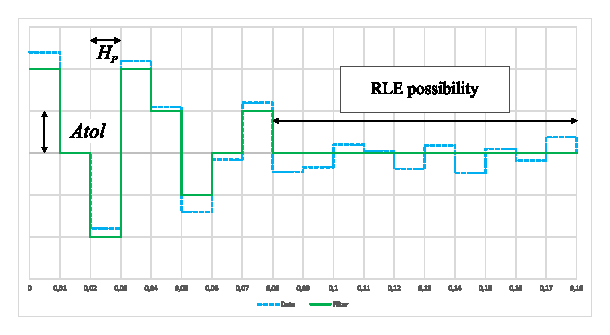
\includegraphics[width=0.8\columnwidth]{fig5.eps}
	\caption{Pre-compression results filtering for RLE in range of \(Atol\).}
	\label{fig_rle}
\end{figure}

In addition, filtering allows to eliminate the effect that may occur when the result values oscillate around zero. 
The IEEE-754 representation of a double-precision number contains sign information in the high bit. 
Slight oscillations in the result values around zero can lead to a sign change. The relatively 
small absolute prediction error, but affecting the sign, will lead to the fact that when encoding \(Z_b\), 
counted from the most significant bits, will be equal to zero, and instead of reducing the size of data, 
the algorithm will increase it, since 4 extra bits will be required for \(Z_b\) encoding. 
Filtering eliminates the sign change caused by oscillations in the results with amplitudes not exceeding 
the \(Atol\), and allows to maintain an acceptable compression ratio.
When \(Atol\) values of \(10^{-4}\) or more are acceptable, which is usually adequate for transient stability
simulation for post-contingency control task, a single precision real number format requiring only 32 bits 
can be used to store the results. 
This will halve the size of results at the cost of accuracy, but at the same time 
retain the ability to use the proposed compression method with minimal changes in the encoding scheme.

\section{Implementation and comparison with mainstream compression algorithms}
To study proposed compression method implementation, series of tests were carried out to store 
transient stability simulation results for the model with the following parameters:

\begin{table}[!h]
	\caption{Test model features\label{tab:testmodel}}
	\centering
	\begin{tabularx}{\columnwidth}{ 
			>{\raggedright\arraybackslash}X 
			| >{\raggedleft\arraybackslash}X }
		\hline
		Equipment model & Count \\
		\hlineB{3}
		Bus & 842 \\
		\hline		
		Branch & 1189 \\
		\hline		
  	    Generator(simplified Park's) & 149 \\
		\hline
		Excitation system (Exciter+AVR+DEC) & 145 \\
		\hline				
	\end{tabularx}
\end{table}

The tests were performed on a PC with an Intel Core i7-4770 CPU 3.4GHz and 32GB of RAM. A 4GB disk drive 
was emulated in RAM, to make file data files I/O times negligible.

The total number of state variables in the model was 6892. 
The Transient with a duration of 100s and a step for the results output \(H_p=10^{-2}s\) in this 
model was simulated for two cases. In the first case (Case 1), the frequency stabilization channels 
of the AVR were switched off, due to which the transient process decayed much more slowly compared to 
the second case (Case 2), in which the AVR stabilization channels were in operation. 
Absolute integration error tolerance were \(Atol=10^{-7}\). Comparison of the simulation results of 
the slip of one of the generators of the model is shown in the figure \ref{fig_cases1}:

\begin{figure}[h]
	\centering
	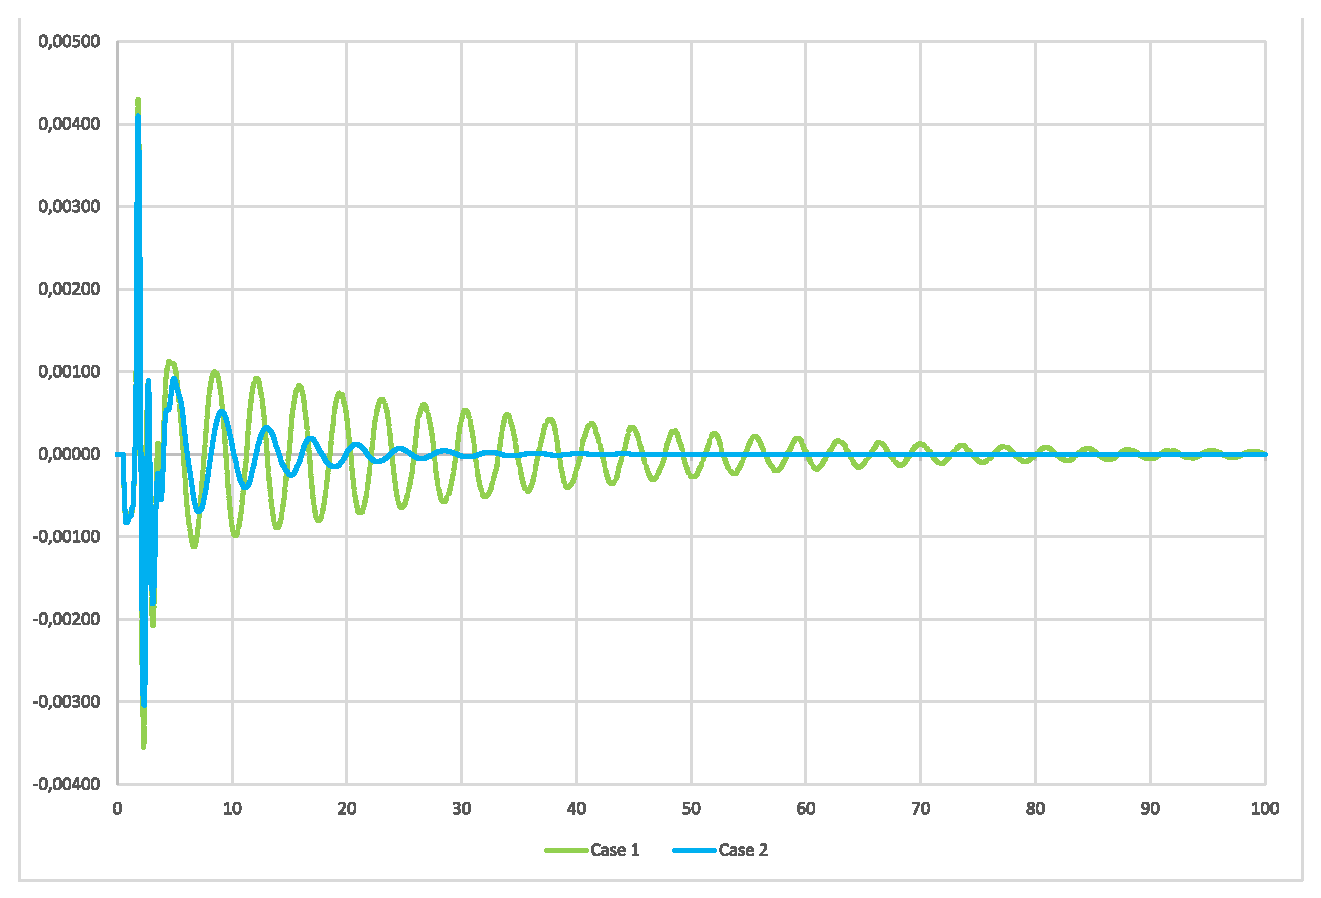
\includegraphics[width=0.8\columnwidth]{fig3.eps}
	\caption{Transient cases with different decays.}
	\label{fig_cases1}
\end{figure}
For Case 2, due to faster decay, the integration method increased the step at the final stage of the
 simulation over \(H_p\), which can be seen from the location of the markers in the 
 figure \ref{fig_cases2}. For that case, therefore, a significantly smaller amount of 
the  results were saved than for Case 1. The resulting sizes were compressed by the proposed method during 
 the simulation. After simulation, the results were restored and compressed by two mainstream 
 archiving programs: WinRAR 5.5 and 7zip 16.02 with maximum compression settings.
 The results of the experiment are shown in the table \ref{tab:winrarz}. The best results are in bold.
  
\begin{figure}[h]
	\centering
	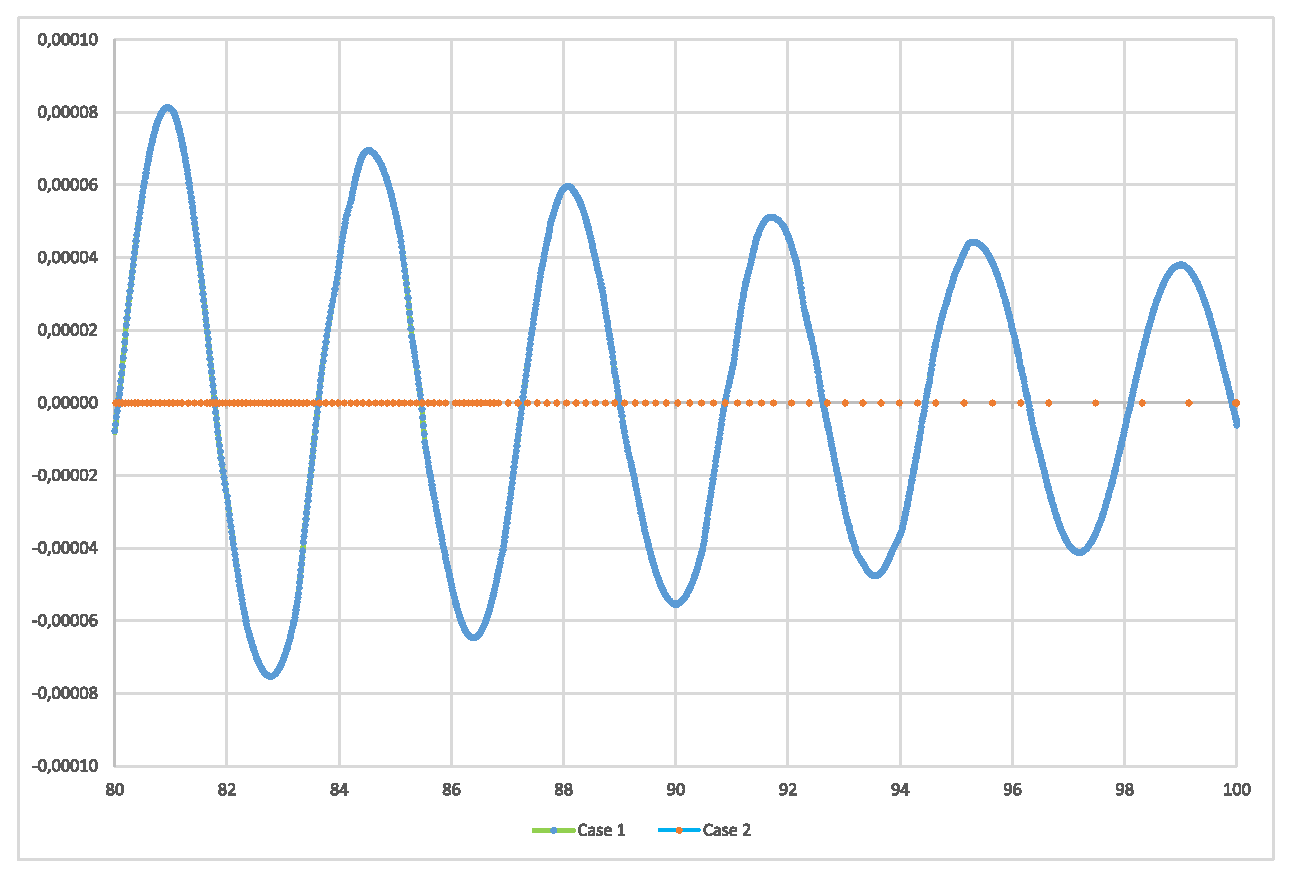
\includegraphics[width=0.8\columnwidth]{fig4.eps}
	\caption{Integration step impact on result output step.}
	\label{fig_cases2}
\end{figure}


\begin{table}[!h]
	\caption{Compression performance comparison\label{tab:winrarz}}
	\centering
	\begin{tabularx}{\columnwidth}{ 
 		     >{\raggedright\arraybackslash}X 
			| >{\raggedleft\arraybackslash}X 
			| >{\raggedleft\arraybackslash}X }
		\hline
 	    & \multicolumn{1}{c|} {Case 1} & \multicolumn{1}{c} {Case 2} \\ 
		\hlineB{3}		
		\multicolumn{3}{c}{Proposed method} \\ 		
		\hline
		Samples count & 8052 & 5298 \\
		\hline
		State vars count & 6892 & 6892 \\
		\hline		
		Uncompressed, MB & 423.39 & 278.58 \\
		\hline
		Time, s & \textbf{16} & \textbf{10} \\
		\hline		
		RAM, GB & \textbf{0.003} & \textbf{0.003} \\
		\hline		
		Compressed, MB & \textbf{169.47} & 102.24 \\
		\hline		
		Ratio, \% & \textbf{40.03} & 36.70 \\
		\hlineB{3}		
		\multicolumn{3}{c}{WinRAR} \\ 		
		\hline		
		Time, s & 19 & 10 \\
		\hline		
		Time 1 core, s &	69 & 38 \\
		\hline		
		RAM, GB & 0.82 & 0.82 \\
		\hline		
		Compressed, MB & 175.20 & \textbf{98.16} \\
		\hline		
		Ratio, \% & 41.38 & \textbf{35.24} \\
		\hlineB{3}		
		\multicolumn{3}{c}{7zip} \\ 	
		\hline	
		Time, s & 38 & 25 \\
		\hline		
		Time 1 core, s & 120 & 62 \\
		\hline		
		RAM, GB & 2.94 & 1.86 \\
		\hline
		Compressed, MB & 197.57 & 106.52 \\
		\hline		
		Ratio, \% & 46.66 & 38.24 \\
		\hline		
	\end{tabularx}
\end{table}

During the comparison, the sizes of the compressed data were measured and the compression ratios were determined, 
, as well as the time spent on the compression. 
The compression ratio of the proposed method turns out to be comparable with the compression ratios of mainstream 
archivers. For a larger amount of results, the proposed method gives the best compression ratio. 
For a smaller size of results, the proposed method is slightly inferior to WinRAR.

It should be noted that in the comparison, the proposed compression method was run in parallel with the process 
of  the transient stability simulation on one core of an eight-core processor. 
The load on the processor from the compression method, thus, could not exceed 12.5\%. 
The WinRAR and 7zip archivers were run with no threading restrictions. 
The average load on the processor when running WinRAR was about 65\%, and when running 7zip --- 53\%. 
In order to compare the time required by that archivers to process data using only one processor core, they 
were artificially restricted by the operating system. The execution time of archivers on one 
processor core is also shown in the table. The amount of memory required by the proposed method is negligible 
compared to the amount required by archivers that use general purpose compression methods.

The "Compressed" row shows the full size of the results compressed by the proposed method, which, 
in addition to these results, also includes auxiliary data, for example, a list of state 
variables with their names and units, a list of model elements, etc., as the compressed size for archivers, 
is only the size of result data. At the end of the comparison, the results compressed 
by the proposed method was additionally compressed by WinRAR. The compression ratio for Case 1 turned out 
to be 96\%, for Case 2 --- 94\%, which can be explained by a better compression of auxiliary data. 
However, compression of the auxiliary data for the result will require 
its full decompression when reading for analysis. Considering that the additional possible compression is negligible, the auxiliary data is stored without using compression to speed up the reading of results.

\section{Conclusion}
The proposed method for compressing the results of transient stability simulation makes it possible to obtain a compression ratio 
close to the compression ratio of mainstream archiving programs that implement general purpose algorithms, with significantly 
less computational efforts. The amount of memory required for the method is several orders of magnitude smaller than the amount 
required for general purpose compression algorithms. The method allows to compress the result of the simulation for each 
state variable separately, therefore, to restore a subset of the data required for analysis, it is not necessary to restore 
the entire amount of data. The method supports a lossy compression option with a normalized error not exceeding the absolute 
integration error tolerance. The results obtained are achieved through the use of specific properties of the data of the results of the 
transient stability simulation. The compression method is implemented as a component of the developed software for 
transient stability simulation.

\begin{thebibliography}{1}
\bibliographystyle{IEEEtran}

\bibitem{lzw77}
J. Ziv and A. Lempel, “A Universal Algorithm for Data Compression”, IEEE Transactions on
Information Theory, Vol. 23, 1977, pp. 337-343.
\bibitem{welch84}
T. A. Welch, "A technique for high-performance data compression", Computer, vol. 17, no. 6, pp. 8-
19, Jun. 1984.
\bibitem{bwt94}
M. Burrows and D. J. Wheeler, “A Block-Sorting Lossless Data Compression Algorithm”, Digital
SRC Research Report 124, 1994.
\bibitem{lch03}
Khalid Sayood, “Lossless Compression Handbook”. Academic Press, 2003, ISBN 0-12-620861-1,
chapter 12.
\bibitem{ratana06}
Ratanaworabhan, J. Ke, and M. Burtscher, "Fast lossless compression of scientific floating-point data,"
in Data Compression Conference, 2006, pp. 133-142.
\bibitem{camata10}
Camata Jose, Burtscher Martin, Barth, William, Coutinho, Alvaro. Accelerating MPI Broadcasts using Floating-Point Compression. 2010

\end{thebibliography}
\newpage
\section{Biography Section}
\vspace{-33pt}
\begin{IEEEbiography}[{
\includegraphics[width=1in,height=1.25in,clip,keepaspectratio]{mashalov}}]{Eugene Mashalov}
Graduated from Electrotechnical Faculty, Ekaterinburg, Urals State Polytechnical University, 1997. 
Received Ph.D degree in 2000 from the same university. 
Works for JSC "Scientific and Technical Center of Unified Power System", Ekaterinburg, Russia.\\
mashalov@gmail.com \\
www.inorxl.com
\end{IEEEbiography}
\vfill
\end{document}


